\documentclass[10pt,a4paper,twoside]{book}

% Packages
\usepackage{hyperref}
\hypersetup{
    hidelinks
}
\usepackage{tocbibind}
\usepackage{amsmath}
\usepackage{graphicx}
\usepackage{multirow}
\usepackage{multicol}
\usepackage{fancyhdr} % For custom headers/footers
\usepackage{geometry} % For page layout adjustments
\geometry{margin=1in}

% Configure fancyhdr
\pagestyle{fancy}
\fancyhf{}
\fancyhead[LE,RO]{\thepage} % Page numbers: left on even, right on odd pages
\fancyhead[RE]{\leftmark}   % Chapter name on even pages (right header)
\fancyhead[LO]{\rightmark}  % Section name on odd pages (left header)

% Title, Author, and Date
\title{Data Privacy Attacks,\\ Cryptography and Data Protection}
\author{Sudeep Kumar Singh, Shubham Kushwaha, Ankit Sarawag}
\date{\today}

\begin{document}

% Title Page
\maketitle

% Preface or Acknowledgements (Optional)
\section*{Preface}
In the contemporary digital age, the security of sensitive data has become a critical concern due to the increasing volume of data exchanged across interconnected systems and the internet. This document explores key concepts surrounding data privacy attacks, cryptographic techniques, and data protection measures. The rise of cyberattacks and the constant evolution of security threats emphasize the need for robust data protection strategies to safeguard personal and organizational information. By focusing on data privacy breaches and cryptographic solutions, this work aims to provide an in-depth understanding of how attacks are executed and what countermeasures can be employed to secure systems. It also covers modern cryptographic techniques such as symmetric and asymmetric algorithms, hash functions, and public-key infrastructure (PKI), which play a vital role in protecting information integrity, confidentiality, and availability. This study is designed to guide students, researchers, and professionals in understanding and mitigating privacy risks and strengthening data security.

\newpage
\section*{Acknowledgements}
We would like to express our deepest gratitude to our professors and mentors at Atma Ram Sanatan Dharma College, Delhi University, for their continuous support, insightful feedback, and encouragement throughout the course of this research. Their guidance in both theoretical and practical aspects of cryptography and data protection has been invaluable. Special thanks to our mentor for providing critical feedback that helped shape our approach to understanding data privacy attacks and cryptographic defenses. We are also thankful for the resources and tools provided by ARSD College, which were instrumental in the successful completion of this work. We would like to extend our appreciation to the authors and researchers whose works have been referenced in this document, especially William Stallings' \textit{Information Privacy Engineering and Privacy by Design}, which provided a comprehensive foundation for understanding privacy threats and regulations. Finally, we acknowledge the contributions of our peers, whose discussions and input have enhanced the quality of this study.


\newpage
\section*{About the Authors}
\subsection*{Sudeep Kumar Singh}
Sudeep Kumar Singh is a third-year student of B.Sc. Computer Science (Hons.) at Atma Ram Sanatan Dharma College, Delhi University. 

\subsection*{Shubham Kushwaha}
Shubham Kushwaha is also a third-year student pursuing B.Sc. Computer Science (Hons.) at Atma Ram Sanatan Dharma College, Delhi University. 

\subsection*{Ankit Sarawag}
Ankit Sarawag, is also a third-year student pursuing B.Sc. Computer Science (Hons.) at Atma Ram Sanatan Dharma College, Delhi University. 

\newpage
\section*{Credits}
\begin{itemize}
    \item \textbf{Sudeep Kumar Singh (28021), Shubham Kushwaha (28090), and Ankit Sarawag (28006)}, students of B.Sc. Computer Science (Hons.) at Atma Ram Sanatan Dharma College, Delhi University, have collaborated on this project.
    
    \item The concepts and theories discussed in this work are based on the book:  
    \textbf{Stallings, William.} \textit{Information Privacy Engineering and Privacy by Design: Understanding Privacy Threats, Technology, and Regulations Based on Standards and Best Practices}. Addison-Wesley Professional, 2019 \cite{Stallings2019}.
    
    \item Resources like \href{https://www.overleaf.com}{Overleaf} and \href{https://www.latex-project.org}{The LaTeX Project} have made it easier to collaborate on documents and manage references effectively.
\end{itemize}





% Table of Contents
\tableofcontents
% Table of Figures
\clearpage
\addcontentsline{toc}{chapter}{List of Figures}
\listoffigures

% Table of Tables
\clearpage
\addcontentsline{toc}{chapter}{List of Tables}
\listoftables
\newpage
% Chapters (No manual counter resets)
\clearpage
\thispagestyle{empty} 
\begin{center}
    \vspace*{\fill} 
    \Huge \textbf{Chapter 1} \\
    \Huge \textbf{Security Attacks}
    \vspace*{\fill}
\end{center}
\clearpage

\chapter{Security Attacks}

\section{Definitions and Key Concepts}
\begin{itemize}
    \item \textbf{Security Attack:} Any action compromising the security of information owned by an organization.
    \item \textbf{Security Mechanism:} A process or device designed to detect, prevent, or recover from a security attack.
    \item \textbf{Security Service:} A service that enhances the security of data processing systems and information transfers, countering security attacks using security mechanisms.
\end{itemize}

\section{Threat vs. Attack}
\begin{itemize}
    \item \textbf{Threat:} Any circumstance or event with the potential to adversely impact organizational operations, assets, individuals, or the nation via unauthorized access, destruction, disclosure, modification of information, and/or denial of service.
    \item \textbf{Attack:} Any malicious activity attempting to collect, disrupt, deny, degrade, or destroy information system resources or the information itself.
\end{itemize}

\section{Types of Security Attacks}

\subsection{Passive Attacks}
\begin{itemize}
    \item \textbf{Nature:} Eavesdropping or monitoring transmissions without affecting system resources.
    \item \textbf{Goals:} Obtain information being transmitted.
    \item \textbf{Types:}
    \begin{itemize}
        \item \textit{Release of Message Contents:} Eavesdropping on communications such as phone conversations, emails, or transferred files.
        \item \textit{Traffic Analysis:} Observing the pattern of messages, frequency, and length without examining the contents.
    \end{itemize}
    \item \textbf{Characteristics:} Difficult to detect; prevention usually involves encryption.
\end{itemize}

\subsection{Active Attacks}
\begin{itemize}
    \item \textbf{Nature:} Involves modification of stored or transmitted data or the creation of false data.
    \item \textbf{Types:}
    \begin{itemize}
        \item \textit{Masquerade:} One entity pretends to be another, often combined with other active attacks.
        \item \textit{Replay:} Passive capture and retransmission of data to produce unauthorized effects.
        \item \textit{Data Modification:} Alteration of legitimate messages or reordering/delaying them to produce unauthorized effects.
        \item \textit{Denial of Service:} Preventing or inhibiting normal use or management of communication facilities, either targeting specific entities or disrupting entire networks.
    \end{itemize}
    \item \textbf{Characteristics:} Detection and recovery are primary goals since absolute prevention is difficult.
\end{itemize}

\begin{figure}[h!]
    \centering
    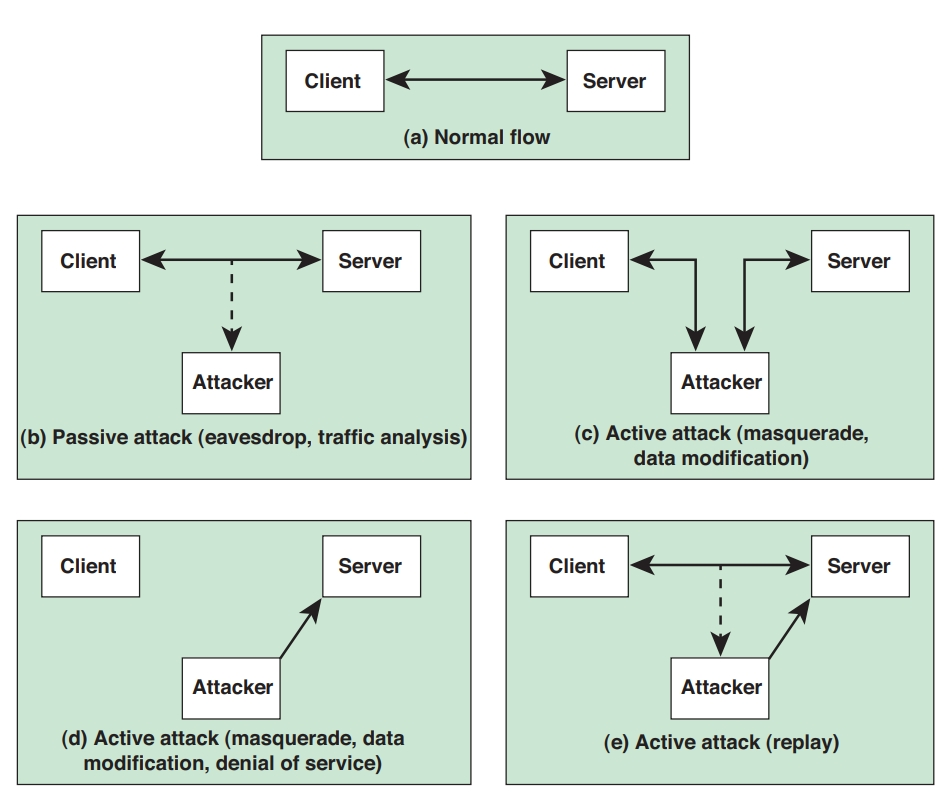
\includegraphics[width=\linewidth]{Data_Privacy_and_Cryptography/Figures/security_attacks.jpeg}
    \caption{Security Attacks}
    \label{fig:security_attacks}
\end{figure}

\section{Illustrations of Security Attacks}
\begin{itemize}
    \item \textbf{Passive Attack Example:} Eavesdropping on client-server communication without disturbing the flow.
    \item \textbf{Active Attack Examples:}
    \begin{itemize}
        \item \textit{Masquerade:} Man-in-the-middle attack, intercepting and pretending to be the client or server.
        \item \textit{Data Modification:} Selectively modifying data communicated between client and server.
        \item \textit{Replay:} Capturing and reusing client messages.
        \item \textit{Denial of Service:} Flooding the server with data or triggering resource-consuming actions.
    \end{itemize}
\end{itemize}

% Chapter Title Page
\clearpage
\thispagestyle{empty} 
\begin{center}
    \vspace*{\fill} 
    \Huge \textbf{Chapter 2} \\
    \Huge \textbf{Security Services} 
    \vspace*{\fill}
\end{center}
\clearpage

\chapter{Security Services}

A security service supports security requirements such as confidentiality, integrity, availability, authenticity, and accountability.\index{Security Service} These services implement security policies using security mechanisms.\index{Security Mechanism}

\section{Key Security Services}
\begin{table}[h!]
    \centering
\begin{tabular}{|p{3.5cm}|p{9cm}|}
    \hline
    \textbf{Service} & \textbf{Description} \\ \hline
    \textbf{Authentication} & Determines a person’s identity before granting access.\index{Authentication} \\ \hline
    \textbf{Access Control} & Limits or allows access to resources for specific purposes.\index{Access Control} \\ \hline
    \textbf{Data Confidentiality} & Ensures information is only available to intended persons.\index{Data Confidentiality} \\ \hline
    \textbf{Data Integrity} & Ensures information is modified only by authorized persons and in appropriate ways.\index{Data Integrity} \\ \hline
    \textbf{Nonrepudiation} & Prevents a person from denying an action they performed.\index{Nonrepudiation} \\ \hline
    \textbf{Availability} & Ensures apps, services, and hardware are ready and perform acceptably when needed.\index{Availability} \\ \hline
\end{tabular}
\caption{Key Security Services}
\end{table}

\section{Authentication}
\begin{itemize}
    \item \textbf{Purpose:} Ensures communication is authentic.\index{Authentication!Purpose}
    \begin{itemize}
        \item \textbf{Single Message:} Ensures the recipient that the message is from the claimed source.\index{Authentication!Single Message}
        \item \textbf{Ongoing Interaction:} Ensures both entities are authentic and the connection is not interfered with.\index{Authentication!Ongoing Interaction}
    \end{itemize}
    \item \textbf{Types of Authentication:}
    \begin{itemize}
        \item \textbf{Peer Entity Authentication:} Confirms the identity of a peer entity in an association, preventing masquerade or unauthorized replay.\index{Peer Entity Authentication}
        \item \textbf{Data Origin Authentication:} Corroborates the source of a data unit, supporting applications like email.\index{Data Origin Authentication}
    \end{itemize}
\end{itemize}

\section{Access Control}
\begin{itemize}
    \item \textbf{Purpose:} Limits and controls access to systems and applications via communications links.\index{Access Control!Purpose}
    \item \textbf{Requirement:} Identification or authentication of each entity to tailor access rights.\index{Access Control!Requirement}
\end{itemize}

\section{Data Confidentiality}
\begin{itemize}
    \item \textbf{Purpose:} Protects transmitted data from passive attacks.\index{Data Confidentiality!Purpose}
    \item \textbf{Protection Levels:}
    \begin{itemize}
        \item Protection of all user data over a connection.\index{Data Confidentiality!User Data Protection}
        \item Protection against traffic flow analysis.\index{Data Confidentiality!Traffic Flow Analysis}
    \end{itemize}
    \item \textbf{Requirement:} Prevents attackers from observing source, destination, frequency, length, or other characteristics of communication.\index{Data Confidentiality!Requirement}
\end{itemize}

\section{Data Integrity}
\begin{itemize}
    \item \textbf{Purpose:} Ensures messages are received as sent, without modification.\index{Data Integrity!Purpose}
    \item \textbf{Types of Integrity Service:}
    \begin{itemize}
        \item \textbf{Connection-Oriented Integrity:} Addresses message stream modification and denial of service for streams of messages.\index{Connection-Oriented Integrity}
        \item \textbf{Connectionless Integrity:} Provides protection against individual message modification.\index{Connectionless Integrity}
    \end{itemize}
\end{itemize}

\section{Nonrepudiation}
\begin{itemize}
    \item \textbf{Purpose:} Prevents sender or receiver from denying transmitted messages.\index{Nonrepudiation!Purpose}
    \begin{itemize}
        \item \textbf{Sender Nonrepudiation:} Receiver can prove the sender sent the message.\index{Sender Nonrepudiation}
        \item \textbf{Receiver Nonrepudiation:} Sender can prove the receiver received the message.\index{Receiver Nonrepudiation}
    \end{itemize}
\end{itemize}

\section{Availability Service}
\begin{itemize}
    \item \textbf{Purpose:} Ensures system or resource is accessible and usable on demand.\index{Availability!Purpose}
    \item \textbf{Requirement:} System provides services as designed whenever users request them.\index{Availability!Requirement}
    \item \textbf{Protection:} Addresses security concerns raised by denial-of-service attacks, depending on access control and other security services.\index{Denial of Service}\index{Availability!Protection}
\end{itemize}

\section{Conclusion}
These security services are essential for maintaining a secure data processing and communication environment in organizations.\index{Security Services!Conclusion}

\thispagestyle{empty}

\begin{center}
    \vspace*{\fill}
    \Huge \textbf{Chapter 3} \\
    \Huge \textbf{Security Mechanisms}
    \vspace*{\fill}
\end{center}

\newpage
\chapter{Security Mechanisms}

\section{Key Security Mechanisms}
Security mechanisms are the methods used to implement security services and ensure the protection of information systems. The key security mechanisms are as follows:

\subsection{Cryptographic Algorithms}
These are techniques used to transform data into a form that is unintelligible to unauthorized parties. Cryptographic algorithms are covered in detail in chapter 4.

\subsection{Data Integrity}
Mechanisms ensuring the integrity of a data unit or stream of data units. These mechanisms verify that data has not been altered during transmission or storage.

\subsection{Digital Signature}
A digital signature is data appended to or a cryptographic transformation of a data unit, allowing the recipient to prove the source and integrity of the data unit. It also protects against forgery by ensuring authenticity.

\subsection{Authentication Exchange}
This mechanism ensures the identity of an entity through the exchange of information, allowing parties to confirm each other’s identity.

\subsection{Traffic Padding}
Traffic padding involves the insertion of bits into gaps in a data stream to obscure the size or frequency of the data, thus frustrating traffic analysis attempts. This makes it harder for attackers to discern patterns in the communication.

\subsection{Routing Control}
Routing control enables the selection of secure routes for data and allows routing changes, especially when a breach of security is suspected. It helps in directing the flow of sensitive information through the most secure channels.

\subsection{Notarization}
Notarization involves a trusted third party that verifies certain properties of a data exchange, ensuring that data has not been tampered with and confirming its authenticity.

\subsection{Access Control}
Access control mechanisms enforce access rights to resources, ensuring that only authorized users or systems can access or modify certain information or resources.


% Chapter Title Page
\clearpage
\thispagestyle{empty} 
\begin{center}
    \vspace*{\fill} 
    \Huge \textbf{Chapter 4} \\
    \Huge \textbf{Cryptographic Algorithms} 
    \vspace*{\fill}
\end{center}
\clearpage

\chapter{Cryptographic Algorithms}

\section{Definitions}

\textbf{Cryptography:} The discipline that involves the principles, means, and methods for transforming data to hide its content, prevent unauthorized use, or undetected modification. It provides information security, including confidentiality, data integrity, non-repudiation, and authenticity.

\textbf{Cryptographic Algorithm:} A well-defined computational procedure related to cryptography that takes variable inputs, often including a cryptographic key, and produces an output.

\section{Categories of Cryptographic Algorithms}

\begin{table}[h]
\centering
\resizebox{\textwidth}{!}{
\begin{tabular}{|p{3.5cm}|p{9cm}|}
\hline
\textbf{Category} & \textbf{Description} \\
\hline
Keyless & Algorithms that do not use any keys during cryptographic transformations. \\

\hline
Single-Key & Algorithms where the transformation result is a function of the input data and a single secret key. \\
\hline
Two-Key & Algorithms that use two related keys (private key and public key) during different stages of the calculation. \\
\hline
\end{tabular}%
}
\caption{Categories of Cryptographic Algorithms}
\end{table}

\section{Keyless Algorithms}

\subsection{Cryptographic Hash Function:} 
Converts a variable amount of text into a small, fixed-length value called a hash value, hash code, or digest. 
\\
It has properties that make it useful in other cryptographic algorithms, such as message authentication codes or digital signatures.

\subsection{Pseudorandom Number Generator:} 
Produces a deterministic sequence of numbers or bits that appear to be random, sufficient for some cryptographic purposes.

\section{Single-Key Algorithms (Symmetric Encryption)}

\subsection{Symmetric Encryption Algorithms:} 
Use a secret key shared between two parties to encrypt and decrypt data. \\This ensures that communication between the parties is protected from outsiders.

\subsection{Message Authentication Code (MAC):} 
A data element generated by a cryptographic transformation involving a secret key and typically a cryptographic hash function of the message. \\It is used to verify the integrity of the message by those possessing the secret key.

\section{Two-Key Algorithms (Asymmetric Encryption)}

\subsection{Asymmetric Encryption Algorithms:} 
Use two related keys: a private key (known only to the user) and a public key (available to others). It can work in two ways:
\begin{itemize}
    \item Encrypting data with the private key and decrypting with the public key.
    \item Encrypting data with the public key and decrypting with the private key.
\end{itemize}

\section{Applications}

\subsection{Digital Signature Algorithm:} 
A value computed with a cryptographic algorithm associated with a data object, used to verify the data's origin and integrity. The signer uses their private key to generate the signature, and anyone with the public key can verify it.

\subsection{Key Exchange:} 
Securely distributing a symmetric key to two or more parties.

\subsection{User Authentication:} 
Authenticating a user attempting to access an application or service and verifying that the service is genuine.

These cryptographic algorithms are fundamental in ensuring the secure storage, transmission, and interaction of data.


% Chapter Title Page
\clearpage
\thispagestyle{empty} 
\begin{center}
    \vspace*{\fill} 
    \Huge \textbf{Chapter 5} \\
    \Huge \textbf{Symmetric Encryption} 
    \vspace*{\fill}
\end{center}
\clearpage
\chapter{Symmetric Encryption}

\section{Definition}
Symmetric encryption, also known as secret-key encryption, is a cryptographic scheme where the same key is used for both encryption and decryption.

\section{Ingredients of Symmetric Encryption}
\begin{figure}
    \centering
    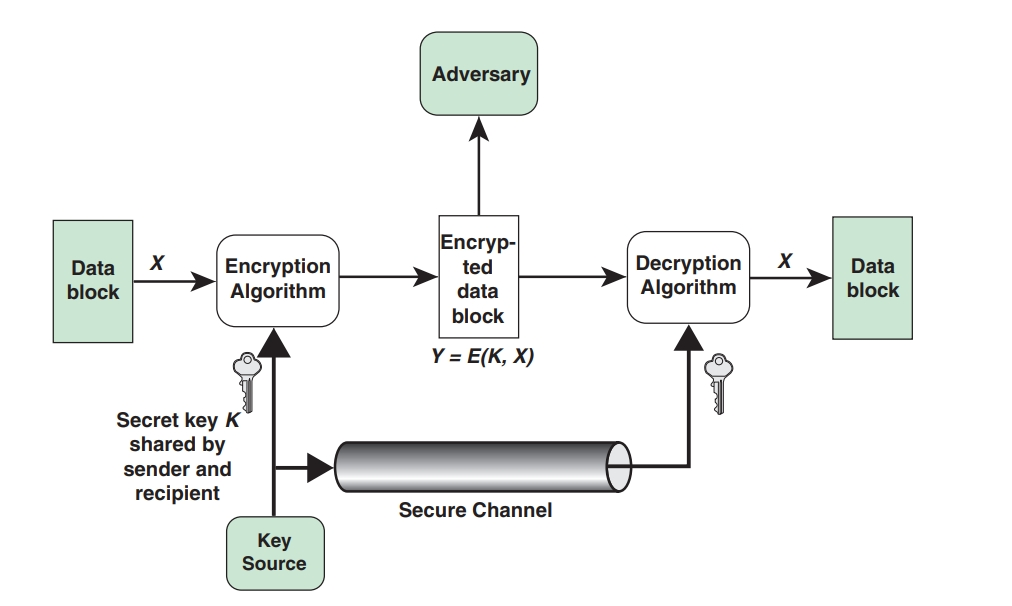
\includegraphics[width=1\linewidth]{Data_Privacy_and_Cryptography/Figures/model of symmetric crypto.jpeg}
    \caption{Model of Symmetric Cryptosystem}
    \label{fig:enter-label}
\end{figure}
\begin{itemize}
    \item \textbf{Plaintext:} The original message or data block that is input into the encryption algorithm.
    \item \textbf{Encryption Algorithm:} The algorithm that performs various substitutions and transformations on the plaintext using the secret key.
    \item \textbf{Secret Key:} An input to the encryption algorithm; the exact substitutions and transformations depend on this key.
    \item \textbf{Ciphertext:} The scrambled message produced as output. It depends on both the plaintext and the secret key. Different keys produce different ciphertexts for the same plaintext.
    \item \textbf{Decryption Algorithm:} The inverse of the encryption algorithm; it uses the ciphertext and the secret key to reproduce the original plaintext.
\end{itemize}

\section{Requirements for Secure Symmetric Encryption}

\begin{itemize}
    \item \textbf{Strong Encryption Algorithm:} 
    \begin{itemize}
        \item The algorithm should be such that an opponent, even with access to the algorithm and multiple ciphertexts, cannot decipher the ciphertext or determine the key.
        \item Ideally, the opponent should not be able to decrypt the ciphertext or discover the key even if they possess multiple ciphertext-plaintext pairs.
    \end{itemize}
    \item \textbf{Secure Key Distribution:} 
    \begin{itemize}
        \item The sender and receiver must obtain copies of the secret key in a secure manner and must keep the key secure.
        \item If an opponent discovers the key, they can read all communications encrypted with that key.
    \end{itemize}
\end{itemize}


\section{Key Generation and Distribution}

A key generation algorithm typically generates a random number and derives a secret key from it.

For two parties to communicate, key distribution can occur through various methods:
\begin{itemize}
    \item One party generates the key and securely transfers it to the other party.
    \item A secure key exchange protocol enables both parties to jointly generate a key known only to them.
    \item A third party generates the key and securely transfers it to the two communicating parties.
\end{itemize}

\section{Potential Adversary Attacks}

\begin{itemize}
    \item \textbf{Cryptanalysis:} 
    \begin{itemize}
        \item Relies on the nature of the algorithm and knowledge of the plaintext or sample plaintext/ciphertext pairs.
        \item  It attempts to deduce the key or specific plaintext.
        \item If successful, all past and future messages encrypted with that key are compromised.
    \end{itemize}
     
    \item \textbf{Brute-Force Attack:}
    \begin{itemize}
        \item  Involves trying every possible key on a piece of ciphertext until an intelligible translation into plaintext is found.
        \item  On average, half of all possible keys must be tried to achieve success.
        \item A secure symmetric encryption scheme requires an algorithm resistant to cryptanalysis and a key of sufficient length to defeat brute-force attacks.
   
    \end{itemize}
\end{itemize}




% Chapter Title Page
\clearpage
\thispagestyle{empty} 
\begin{center}
    \vspace*{\fill} 
    \Huge \textbf{Chapter 6} \\
    \Huge \textbf{Asymmetric Encryption} 
    \vspace*{\fill}
\end{center}
\clearpage
\chapter{Asymmetric Encryption}

\section{Definition}
Public-key cryptography, also known as asymmetric cryptography, uses two separate keys for encryption and decryption. This contrasts with symmetric encryption, which uses only one key.

\section{Ingredients of Asymmetric Encryption}
\begin{figure}
    \centering
    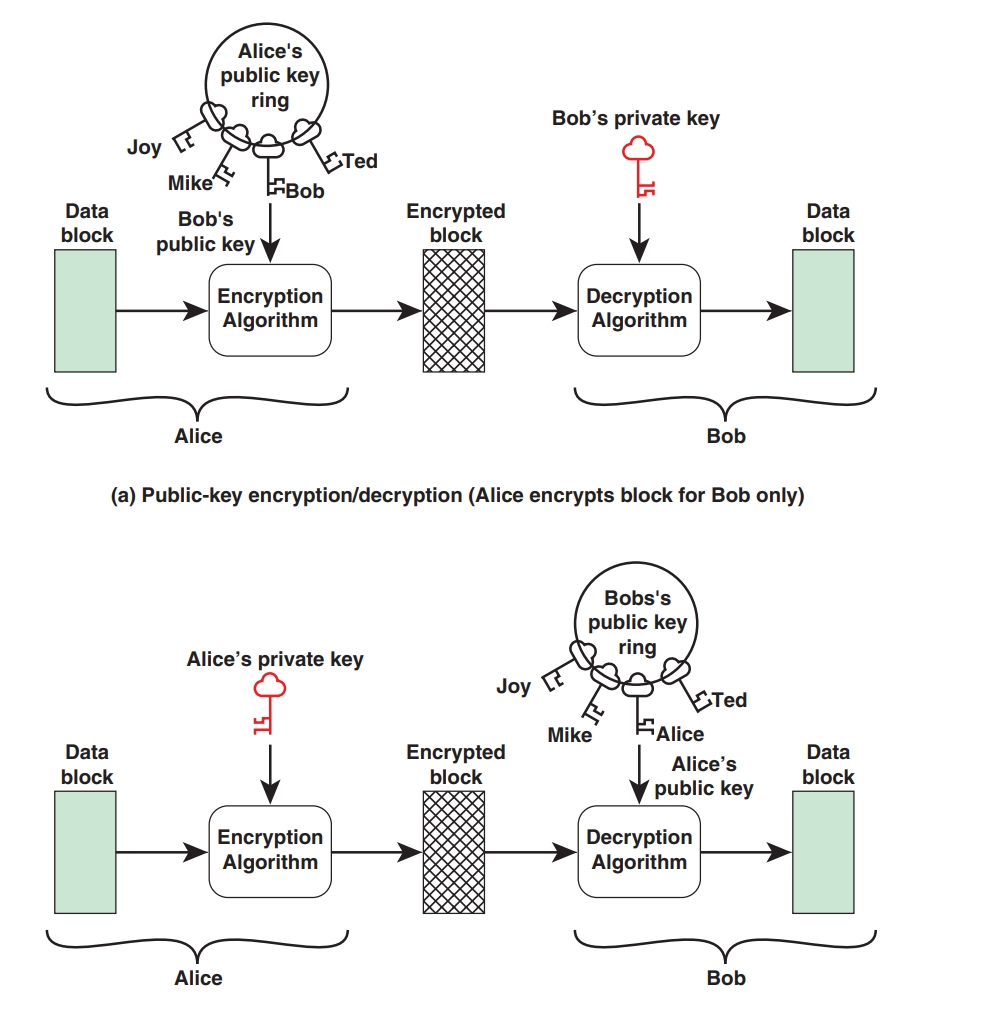
\includegraphics[width=1\linewidth]{Data_Privacy_and_Cryptography/Figures/model of asymmetric crypto.jpeg}
    \caption{Model of Asymmetric Cryptosystem}
    \label{fig:asymmetric}
\end{figure}
\begin{itemize}
    \item \textbf{Plaintext:} The readable message or data block input into the encryption algorithm.
    \item \textbf{Encryption Algorithm:} Performs various transformations on the plaintext using a key.
    \item \textbf{Public Key and Private Key:} A pair of keys selected such that if one key is used for encryption, the other is used for decryption. The transformations depend on the key used.
    \item \textbf{Ciphertext:} The scrambled block produced as output, depending on the plaintext and the key used.
    \item \textbf{Decryption Algorithm:} The inverse of the encryption algorithm, it accepts the ciphertext and the matching key to produce the original plaintext.
\end{itemize}

\section{Process of Asymmetric Encryption}

\begin{itemize}
    \item \textbf{Key Generation:} Each user generates a pair of keys (public and private) for encryption and decryption.
    \item \textbf{Public Key Sharing:} One of the keys (public key) is placed in a public register or accessible file, while the companion key (private key) is kept secret.
    \item \textbf{Encryption:} If Alice wants to send a confidential message to Bob, she encrypts the message using Bob’s public key.
    \item \textbf{Decryption:} Bob decrypts the message using his private key. No one else can decrypt the message because only Bob knows his private key.
\end{itemize}

\section{Comparison with Symmetric Encryption}
\begin{table}[h!]
    \centering
\begin{tabular}{|p{6.5cm}|p{6.5cm}|}
\hline
\textbf{Symmetric Encryption} & \textbf{Asymmetric Encryption} \\
\hline
Uses the same algorithm with the same secret key for encryption and decryption. & Uses one algorithm for encryption and a related algorithm for decryption, with a pair of keys (public and private). \\
\hline
Sender and receiver must share the algorithm and the secret key. & Sender and receiver must each have a unique public/private key pair. \\
\hline
Key must be kept secret. & Private key must be kept secret. \\
\hline
Algorithm plus samples of ciphertext must be insufficient to determine the key. & Algorithm plus public key plus samples of ciphertext must be insufficient to determine the private key. \\
\hline
\end{tabular}
\caption{Symmetric Vs Asymmetric Encryption}
\end{table}
\section{Alternative Uses}

\begin{itemize}
    \item \textbf{Authentication:} 
    \\
    Alice can use her private key to encrypt a message. When Bob decrypts it with Alice’s public key, he can be certain the message came from Alice.
\end{itemize}

\section{Security Considerations}
The security of public-key encryption relies on the strength of the algorithm and the length of the private key. 
\\
Public-key cryptographic algorithms are generally slower than symmetric algorithms and are often limited to small blocks of data, such as a secret key or a hash value.

% Chapter Title Page
\clearpage
\thispagestyle{empty} 
\begin{center}
    \vspace*{\fill} 
    \Huge \textbf{Chapter 7} \\
    \Huge \textbf{Cryptographic Hash Functions} 
    \vspace*{\fill}
\end{center}
\clearpage

\chapter{Cryptographic Hash Functions}

\section{Definition}
A hash function takes an input of arbitrary length and maps it to a fixed-length data block. Multiple input blocks may produce the same output, known as the hash value or hash digest.

\section{Requirements for Cryptographic Hash Function}

\begin{table}[h!]
\centering
\begin{tabular}{|p{3.5cm}|p{9cm}|}
\hline
\textbf{Requirement} & \textbf{Description} \\
\hline
Variable input size & Can be applied to a block of data of any size. \\
\hline
Fixed output size & Produces a fixed-length output. \\
\hline
Efficiency & Relatively easy to compute for any given input, making hardware and software implementations practical. \\
\hline
Preimage resistant & Computationally infeasible to find an input that maps to a given hash value. \\
\hline
Second preimage resistant & Computationally infeasible to find a different input with the same hash value. \\
\hline
Collision resistant & Computationally infeasible to find any two different inputs that map to the same hash value. \\
\hline
Pseudorandomness & Output appears to be a random sequence of bits. \\
\hline
\end{tabular}
\caption{Requirements for Cryptographic Hash Function}
\end{table}
\begin{figure}
    \centering
    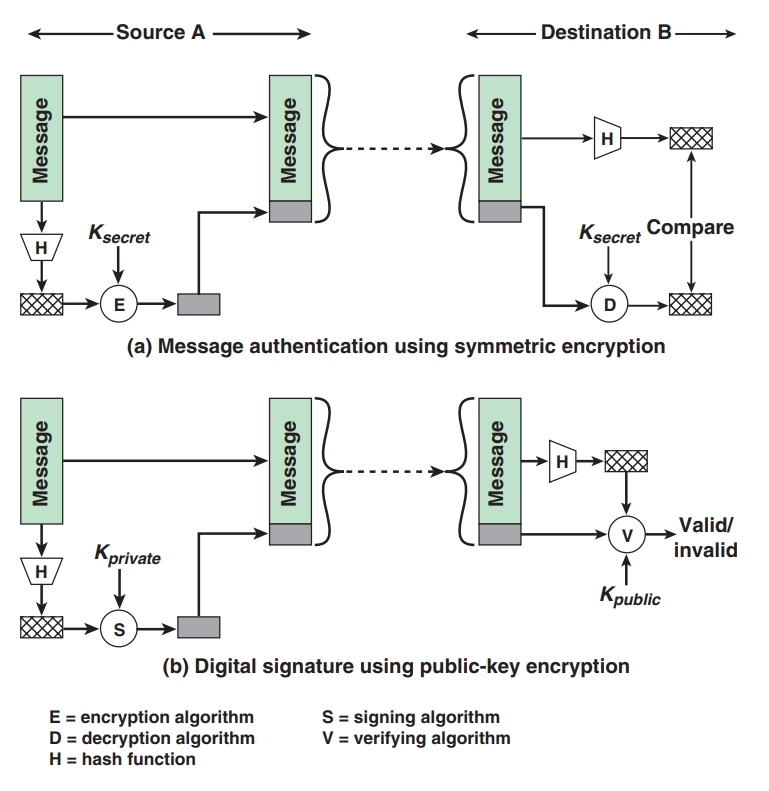
\includegraphics[width=1\linewidth]{Data_Privacy_and_Cryptography/Figures/use of secure hash fun.jpeg}
    \caption{Uses for a Secure Hash Function}
    \label{fig:hashfunction}
\end{figure}


\section{Uses of Cryptographic Hash Functions}

\subsection{Message Authentication:}
Ensures data integrity and verifies the authenticity of the message source. 

Example process:
\begin{enumerate}
    \item Generate a hash value for the source message.
    \item Encrypt the hash value using a secret key shared by a cooperating partner.
    \item Transmit the message plus the encrypted hash value to the destination.
    \item The recipient decrypts the hash value, generates a new hash value from the incoming message, and compares the two hash values.
\end{enumerate}

\subsection{Digital Signatures:}
Verifies the origin and integrity of a message. The sender's private key is used to encrypt the hash value, and the recipient can use the sender's public key to decrypt it and verify the message.

\section{Digital Signatures}

\subsection{Definition:}
A cryptographic transformation of data ensuring origin authentication, data integrity, and non-repudiation (NIST FIPS 186-4).

\subsection{Process:}
\begin{enumerate}
    \item \textbf{Hash Generation:} Bob generates a hash value for his message using a secure hash function.
    \item \textbf{Signature Creation:} Bob uses his private key and the hash value to create a digital signature.
    \item \textbf{Sending:} The message is sent with the digital signature attached.
    \item \textbf{Verification:} \begin{enumerate}
    \item The receiver generates a hash value of the received message.
    \item The receiver uses Bob’s public key, the generated hash, and the received signature to verify the message.
    \item If valid, it confirms the message was indeed sent by Bob and hasn’t been altered.
\end{enumerate}
\end{enumerate}


\subsection{Applications:}
\begin{itemize}
    \item Signing email messages for sender authentication.
    \item Signing software programs to authenticate their source and counter software tampering.
    \item Verifying authorship or origin of digital data.
    \item Ensuring the integrity of digital data against tampering.
    \item Authenticating online entities.
\end{itemize}


\renewcommand{\footrulewidth}{0.5pt}
\fancyfoot[LO,RE]{\small
    \textbf{NIST\textsuperscript{1}:} National Institute of Standards and Technology, 
    \textbf{FIPS\textsuperscript{2}:} Federal Information Processing Standards, 
    \textbf{SP\textsuperscript{3}:} Special Publication, 
    \textbf{ENISA\textsuperscript{4}:} European Union Agency for Cybersecurity, 
    \textbf{SHA\textsuperscript{5}:} Secure Hash Algorithm, 
    \textbf{RSA\textsuperscript{6}:} Rivest-Shamir-Adleman,  
    \textbf{DSA\textsuperscript{7}:} Digital Signature Algorithm,  
    \textbf{ECDSA\textsuperscript{8}:} Elliptic Curve Digital Signature Algorithm
}


% Chapter Title Page
\clearpage
\thispagestyle{empty} 
\begin{center}
    \vspace*{\fill} 
    \Huge \textbf{Chapter 8} \\
    \Huge \textbf{Practical Considerations} 
    \vspace*{\fill}
\end{center}
\clearpage

\chapter{Practical Considerations}

\section{Cryptographic Algorithms and Key Lengths}

\subsubsection{Security Over Time:}
\begin{itemize}
    \item Processor speeds and scrutiny increase over time, which can lead old algorithms to become insecure.
    \item Key lengths and hash values that were secure before may now be too weak due to increased computational power and analysis techniques.
\end{itemize}

\subsection{Guidance Sources:}
\begin{itemize}
    \item \textbf{FIPS\textsuperscript{2} 140-2A:} Approved Security Functions for FIPS PUB 140-2.
    \item \textbf{SP\textsuperscript{3} 800-131A:} Transitioning the Use of Cryptographic Algorithms and Key Lengths.
    \item \textbf{ENISA\textsuperscript{4}:} Algorithms, Key Size, and Protocol Report [ECRY18].
\end{itemize}

\subsection{Recommendations:}
\begin{enumerate}
    \item \textbf{Symmetric Encryption:}
    \begin{itemize}
        \item \textbf{Advanced Encryption Standard (AES):} Key lengths of 128, 192, or 256 bits.
    \end{itemize}
    \item \textbf{Hash Functions:}
    \begin{itemize}
        \item \textbf{SHA\textsuperscript{5}-2 or SHA-3:} Hash lengths range from 224 to 512 bits.
    \end{itemize}
    \item \textbf{Digital Signatures:}
    \begin{itemize}
        \item \textbf{Digital Signature Algorithm (DSA)\textsuperscript{7}:} 2048 bits.
        \item \textbf{RSA\textsuperscript{6} Algorithm:} 2048 bits.
        \item \textbf{Elliptic-Curve Digital Signature Algorithm (ECDSA)\textsuperscript{8}:} 224 bits.
    \end{itemize}
\end{enumerate}

\subsection{Implementation Considerations:}
\begin{itemize}
    \item \textbf{Standards Selection:}
    \begin{itemize}
        \item Rely on standardized algorithms (e.g., AES, SHA, DSS).
        \item Use standards developed by \textbf{NIST\textsuperscript{1}} and other trusted organizations.
    \end{itemize}
    \item \textbf{Implementation Methods:}
    \begin{itemize}
        \item Choose between hardware, software, and firmware based on security, cost, simplicity, efficiency, and ease of implementation.
    \end{itemize}
    \item \textbf{Key Management:}
    \begin{itemize}
        \item Administer and manage cryptographic keys (generation, protection, storage, etc.).
        \item For more details, refer to \textit{Effective Cybersecurity: Best Practices and Standards [STAL19]}.
    \end{itemize}
    \item \textbf{Cryptographic Module Security:}
    \begin{itemize}
        \item Secure design, implementation, and use of cryptographic modules.
        \item Use \textbf{NIST\textsuperscript{1}} Cryptographic Module Validation Program (CMVP) for validation.
    \end{itemize}
\end{itemize}

\section{Lightweight Cryptographic Algorithms}

\subsection{Focus:}
\begin{itemize}
    \item Develop secure algorithms minimizing execution time, memory usage, and power consumption.
    \item Suitable for embedded systems (e.g., IoT devices).
\end{itemize}

\subsection{NIST Project:}
\begin{itemize}
    \item \textbf{NIST \textsuperscript{1}} is working on developing a portfolio of lightweight algorithms.
    \item Initial focus is on symmetric encryption and secure hash functions.
\end{itemize}

\section{Post-Quantum Cryptographic Algorithms}

\subsubsection{Concerns:}
\begin{itemize}
    \item Quantum computers may break current asymmetric cryptographic algorithms, leading to vulnerabilities.
\end{itemize}

\subsection{NIST Effort:}
\begin{itemize}
    \item \textbf{NIST\textsuperscript{1}} is working on standardizing algorithms that can replace or complement existing asymmetric cryptographic schemes.
    \item They are exploring mathematical approaches for new asymmetric cryptographic algorithms resistant to quantum computing threats.
\end{itemize}

% Chapter Title Page
\clearpage
\thispagestyle{empty} 
\begin{center}
    \vspace*{\fill} 
    \Huge \textbf{Chapter 9} \\
    \Huge \textbf{Public-Key Infrastructure (PKI)}
    \vspace*{\fill}
\end{center}
\clearpage
\fancyfoot[]{}
\chapter{Public-Key Infrastructure (PKI)}

\section{Definition:}
\begin{itemize}
    \item PKI supports the distribution and identification of public encryption keys.
    \item It enables secure data exchange over networks and verifies the identity of the other party.
    \item PKI binds public keys to entities and manages public key bindings.
\end{itemize}

\section{Public-Key Certificates:}
\begin{itemize}
    \item A public-key certificate is a set of data that uniquely identifies an entity, containing the entity’s public key and other data.
    \item It is digitally signed by a trusted party, known as the Certification Authority (CA), binding the public key to the entity.
    \item The certificate solves the problem of public-key distribution by ensuring authenticity.
\end{itemize}

\section{Certificate Generation and Use:}
\begin{itemize}
    \item \textbf{Certificate Components:}
    \begin{itemize}
        \item Contains unique identifying information for the entity.
        \item Public key of the entity.
        \item Information about the CA.
        \item Certificate details (e.g., expiration date).
    \end{itemize}
    \item \textbf{Signing:}
    \begin{itemize}
        \item Information is hashed, and a digital signature is generated using the CA’s private key.
        \item The certificate is signed and can be broadcast or attached to documents.
    \end{itemize}
    \item \textbf{Verification:}
    \begin{itemize}
        \item Users verify the certificate's validity using the CA’s public key.
        \item Ensures the public key in the certificate is authentic.
    \end{itemize}
\end{itemize}
\begin{figure}
    \centering
    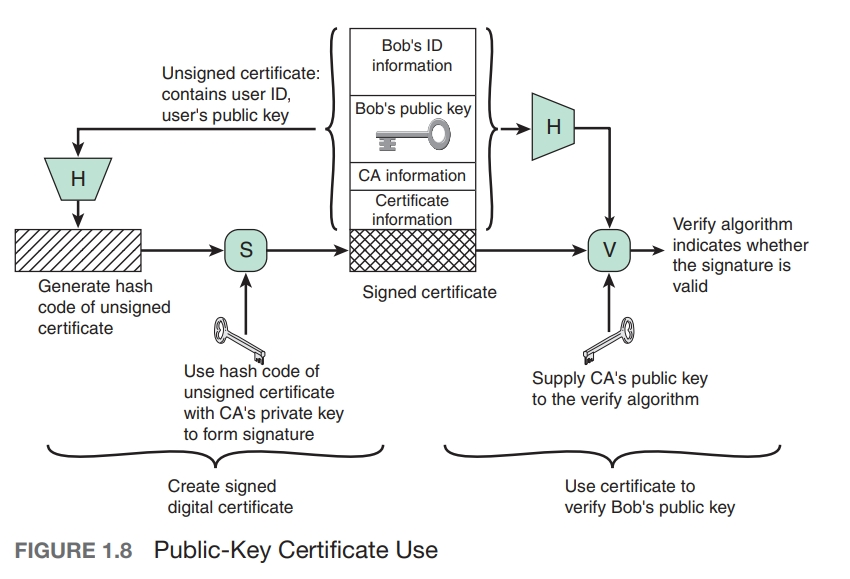
\includegraphics[width=1\linewidth]{Data_Privacy_and_Cryptography/Figures/public key certificate use.jpeg}
    \caption{Public-Key Certificate Use}
    \label{fig:pkcertificate}
\end{figure}
\section{PKI Architecture:}

\subsection{Requirements:}
\begin{itemize}
    \item Any participant can read and verify a certificate’s owner and authenticity.
    \item Only the CA can create and update certificates.
    \item Participants can verify the current validity of certificates.
\end{itemize}
\begin{figure}
    \centering
    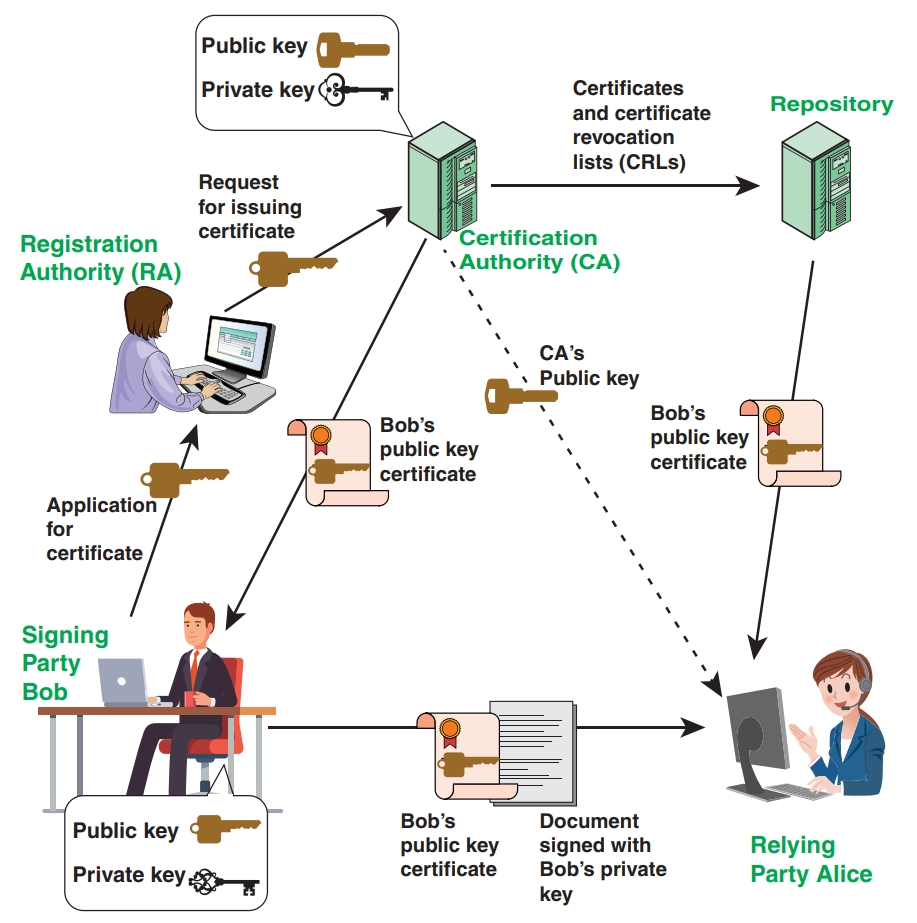
\includegraphics[width=1\linewidth]{Data_Privacy_and_Cryptography/Figures/PKI Scenario.jpeg}
    \caption{PKI Scenario}
    \label{fig:pkiscenario}
\end{figure}
\subsection{Components:}
\begin{itemize}
    \item \textbf{End Entity:} Users, devices, or processes identified in certificates.
    \item \textbf{Certification Authority (CA):} Creates and assigns certificates, issues certificate revocation lists (CRLs).
    \item \textbf{Registration Authority (RA):} Optional, offloads administrative functions from the CA, verifies end entity identity.
    \item \textbf{Repository:} Stores and retrieves PKI-related information (certificates and CRLs).
    \item \textbf{Relying Party:} Users or agents relying on certificate data for decision-making.
\end{itemize}

\section{Certificate Use Example:}
\begin{itemize}
    \item Alice needs Bob’s public key.
    \item Alice obtains the CA’s public key securely.
    \item Alice checks the repository for Bob’s certificate and verifies its validity.
    \item Alice encrypts data to Bob using Bob’s public key.
    \item Bob can send a signed document to Alice, who verifies the signature with Bob’s public key.
\end{itemize}

\section{Hierarchical CA Organization:}
\begin{itemize}
    \item Multiple CAs can be organized hierarchically, with a root CA signing subordinate CAs.
    \item Root certificates are embedded in browsers and other software for built-in trust.
\end{itemize}


\end{document}
